






% =========----------	[ Space left here for distraction free mode] ----------==========%









\subsection{Analysis 1: Does viewing position affect spatial attribute scores?}
	\label{ana1}

		% Ana1 Intro
		To measure the effect that viewing from a different position within the room might have on the participants perception of the given spatial attributes, the test data was split into four groups containing the average results for each spatial attribute, each of which was split into two sub groups corresponding to the data obtained when viewing from position A or B. The data is illustrated in figure~\ref{image:AvsB}.

		It can be seen that the average spatial attribute scores for viewing position A and B are close with the difference in overall mean score being 0.02. Running a Two-Sample T-Test between each of the four spatial attribute groups (e.g A vs B for locatedness etc) indicates no statistical significance. Running the same test for the averaged combined spatial attribute score (average of all four spatial attribute scores) also indicates no statistical significant between viewing position. This is made clear in figure \ref{image:AvsB_dist} illustrating the overall similarity in the distribution of scores for viewing position A and B. \\
		\begin{figure}
			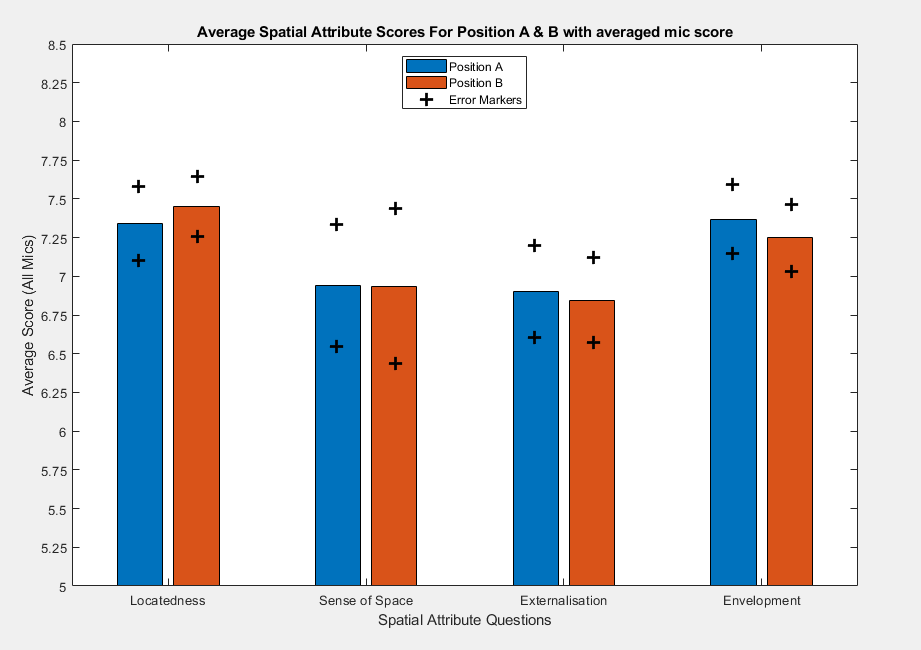
\includegraphics[width=0.5\textwidth]{images/plots/AvB_Bar_error.PNG}
			\caption{Bar chart showing average spatial attribute score for each spatial attribute at viewing position A and B}
			\label{image:AvsB} 
		\end{figure}
		
		% NOTE: Should I display the distributiong as 'normal' or 'kernel'?
		\begin{figure}[t]
			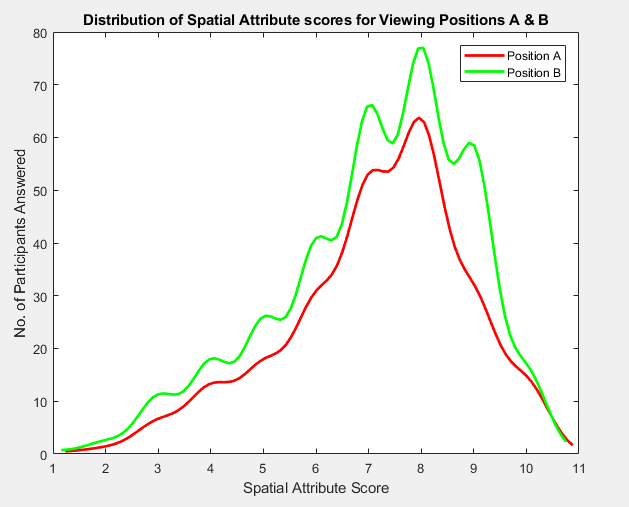
\includegraphics[width=0.5\textwidth]{images/stats/AvsB_sa_stack_all.PNG}
			\caption{Histogram showing the distribution of spatial attribute scores for viewing position A and B. This indicates that viewing position has little effect on spatial qualities in a VR environment.}
			\label{image:AvsB_dist} 
		\end{figure}

		\textbf{Conclusion}\\

		The bar chart indicates that the average spatial attribute scores are extremely close with an overall average for both being 7.1. The Two-Sample T-Test returned $p > 0.05$ for all data groups indicating that the probability of these results recurring is not unlikely and therefore the results shown are not statistically significant.

